\section{Decisiones de dise�o} \label{decisiones}

\subsection{Lenguaje de programaci�n y sistema operativo elegido}
Para implementar el sistema, se ha decidido utilizar el lenguaje de programaci�n Python (\cite{Python}), en un sistema operativo UNIX.

Se ha seleccionado este lenguaje de programaci�n ya que permite el uso de estructuras como diccionarios (tablas hash), listas, manejadores de archivos, llamadas al sistema, definici�n de patrones mediante expresiones regulares, etc. Dichos elementos han facilitado el desarrollo de este m�dulo del sistema, ya que Python los gestiona de una manera eficaz y permite su uso de uso de una manera sencilla.

Por otra parte, 

\subsection{Dise�o de la base de datos}

Para implementar los elementos necesarios para la indexaci�n de documentos, como son el \textit{Posting$\_$File}, la tabla de documentos y el diccionario de t�rminos, se ha optado por utilizar una base de datos relacional, siguiendo el diagrama mostrado en la Figura \ref{BD}. Las tablas que se representan son:

\begin{milista}
	\item \textbf{dic}: implementa el diccionario de t�rminos. Tiene los campos \textit{term} y \textit{num$\_$docs}, que representan cada uno de los t�rminos encontrados, junto con el n�mero de documentos donde aparece cada t�rmino.
	\item \textbf{doc}: implementa la tabla de documentos. Tiene los campos \textit{id$\_$doc}, \textit{title} y \textit{path} para almacenar un identificador �nico de documento, el t�tulo del documento y la ruta del sistema donde se almacena una copia de dicho documento. 
	\item \textbf{posting$\_$file}: implementa el posting$\_$file. Contiene los campos \textit{term}, \textit{id$\_$doc} y \textit{frequency} para representar la frecuencia con la que aparece un t�rmino en un documento. Por tanto, el campo \textit{term} hace referencia a t�rminos del diccionario, y el campo \textit{id$\_$doc} hace referencia a los documentos de la tabla de documentos.
\end{milista}

\begin{figure}[!tb]
	\centering
		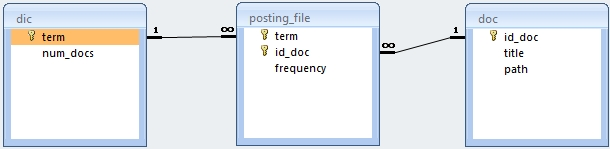
\includegraphics[keepaspectratio]{BD}
	\caption{Diagrama de la base de datos}
	\label{fig:organigrama}
\end{figure} 

